\documentclass[14pt,A4]{extarticle}

\usepackage[utf8]{inputenc}

\usepackage{fontspec}
\setmainfont[Ligatures=TeX]{Times New Roman}
\usepackage[russian]{babel}
\usepackage[a4paper]{geometry}
\geometry{top=2cm, bottom=2cm, left=3cm, right=2cm}

\usepackage{multicol}
\usepackage{multirow}

\usepackage{array}

\usepackage{graphicx}
\graphicspath{{data/}}

\usepackage{indentfirst}
\usepackage{longtable}

\usepackage{float}

\usepackage{listings}

\usepackage{amsmath}
\usepackage{amssymb}
\usepackage{amstext}

\lstset
{
 frame = tb,
 keepspaces = true,
 inputencoding = utf8,
 extendedchars=\true,
 columns = flexible,
 showstringspaces = true,
 basicstyle = {\fontspec{Lucida Console}},
 numbers = left,
 firstnumber = 1,
 breaklines=true,
 breakatwhitespace=true,
 language=C++,
 escapeinside=||
}

\linespread{1.3}

\begin{document}
 \begin{titlepage}
  \begin{center}
  {\fontsize{10}{12}\selectfont \bf
  МИНИСТЕРСТВО НАУКИ И ВЫСШЕГО ОБРАЗОВАНИЯ РОССИЙСКОЙ ФЕДЕРАЦИИ\\
  федеральное государственное автономное образовательное учреждение высшего образования\\
  
  <<Университет>>}
  
  \vspace{1cm}
  Факультет
  
  \vspace{1cm}
  Кафедра 
  
  \vspace{2cm}
  Контрольная работа по дисциплине: \\
  <<  >>\\
  
  На тему: <<  >> \\
  \vspace{2cm}
  
  \begin{tabular}{m{10cm} m{10cm}}
    & Работу выполнил студент\\
    & Группы \\
    &  \\
    & Номер зачетной книжки:\\
    &  \\
    & \\
    & Проверил:\\
    &  \\
    &  \\
  \end{tabular}

  \vspace{2cm}
  Город \\
  year
 \end{center}
  \end{titlepage}

  \tableofcontents
  
  \newpage



\section*{Введение}
\addcontentsline{toc}{section}{Введение}





\newpage

\section{Section1}

\subsection{section1.1}

\subsubsection{section1.1.1}

text

\subsubsection{section1.1.2}

\begin{itemize}
 \item
 \item
 \item
\end{itemize}

\vspace{10mm}

text



\subsection{section1.2}

\begin{figure}[H]
 \centering
 
\includegraphics[height=8cm]{img/test1}
 \caption{test}
 \label{fig:image}
\end{figure}



\newpage

\section{Section2}

\subsection{section2.1}

\begin{figure}[H]
 \centering
 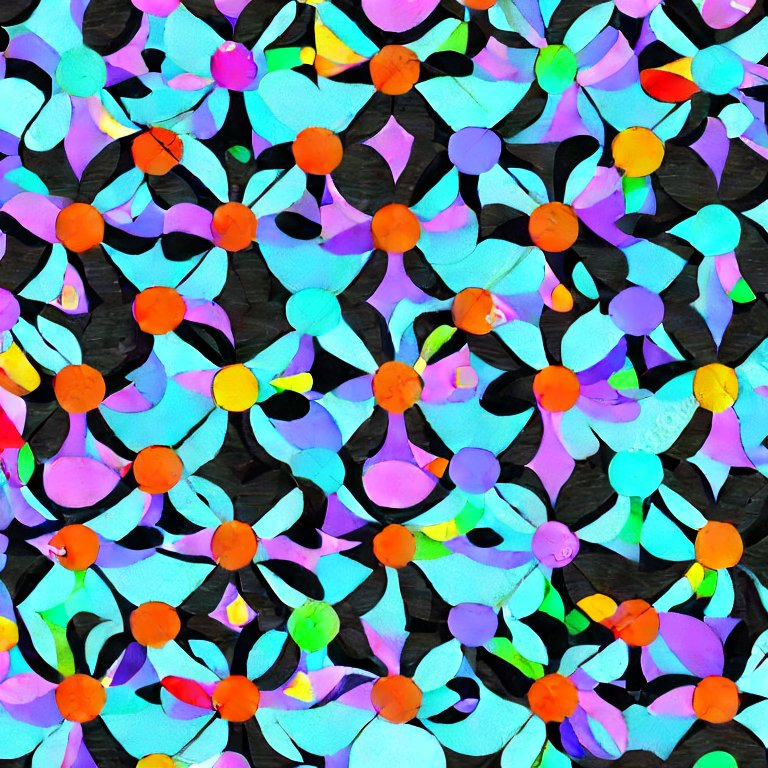
\includegraphics[height=8cm]{img/test2}
 \caption{test}
 \label{fig:image}
\end{figure}



\subsection{section2.2}

\noindent\begin{tabular}{|l|l|l|}
  \hline
  Наименование реквизита&Идентификатор&Формат \\
  \hline
  1&2&3 \\
  \hline
  Идентификатор&id&bigint \\
  \hline
  Наименование&name&varchar(255) \\
  \hline
 \end{tabular}



\newpage

\section*{Заключение}
\addcontentsline{toc}{section}{Заключение}

\newpage

\section*{Список литературы}
\addcontentsline{toc}{section}{Список литературы}

\begin{enumerate}
 \item 
 \item 
 \item 
\end{enumerate}



\newpage

\section*{Приложения}
\addcontentsline{toc}{section}{Приложения}

Приложение 1. code example

\addcontentsline{toc}{subsection}{code example}

\lstinputlisting{data/codeexample.txt}


\end{document}
